\documentclass[12pt]{article}
\usepackage[T1]{fontenc}
\usepackage{mathptmx}
\usepackage{graphicx}
\graphicspath{ {mainpackage/gen600}{screenshots/} }

\begin{document}
\begin{center}
Introduction to Artificial Intelligence – Laboratory 1

Paweł Wiśniewski 232540
\end{center}

\section{Source code}

\subsection{Task generator}
\begin{center}
	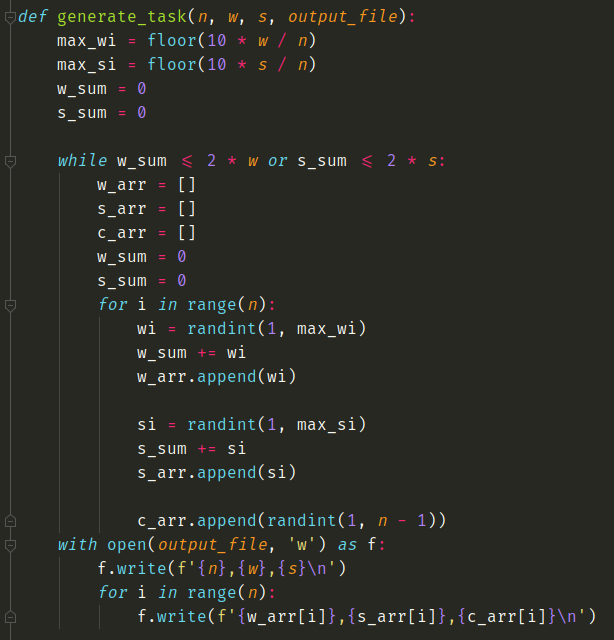
\includegraphics[scale=0.5]{gentask}
\end{center}

In the beginning, the function calculates the maximum weight and size for a single item.
After that, it randomly chooses parameters for each item. The while loop repeats that process until the given criteria are met.
My observations show that in almost all cases the requirements are satisfied after the first iteration.
Finally, results are being written to the given file in the desired format.


\subsection{Item class}
\begin{center}
	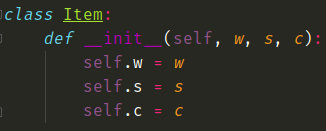
\includegraphics[scale=0.5]{item}
\end{center}

Item class consists of a simple constructor, that saves informations about items weight, size and cost.

\subsection{Task class}
\begin{center}
	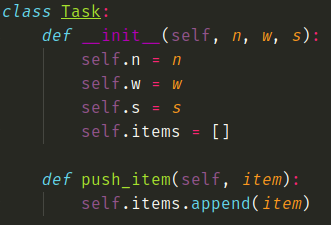
\includegraphics[scale=0.5]{task}
\end{center}

Task class consists of a simple constructor, that saves informations about the number if items, maximum weight and size. In addition, it
initializes an empty list designed for storing items. The class has a \emph{push\_item} method, that simplifies the insertion of items.

\subsection{Task loading}
\begin{center}
	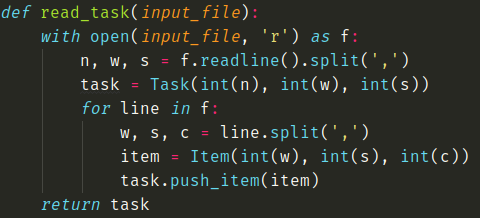
\includegraphics[scale=0.5]{readtask}
\end{center}

The task is loaded from a csv file. The first line contains informations about the number of items, the maximum weight and size.
There are saved in an object of the Task class. The rest of the lines represents items and theirs parameters. The data are stored as the objects of the Item class and pushed to the task object. All the numbers are converted to integers.


\subsection{Population class}

\subsubsection{Constructor}
\begin{center}
	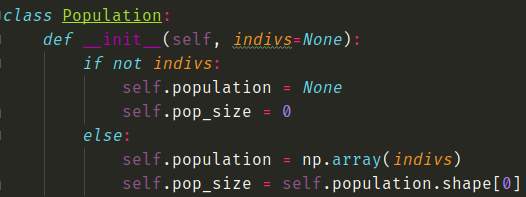
\includegraphics[scale=0.5]{pop_constr}
\end{center}

The constructor uses a parameter \emph{indivs} to pass a list of individuals. That list is converted into NumPy array (NumPy is a
 powerful package for scientific computing with Python).
If no individuals are provided, an empty population is created. 


\subsubsection{Get individual by id method}
\begin{center}
	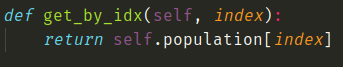
\includegraphics[scale=0.5]{pop_get_by_idx}
\end{center}

This method simplifies the process of obtaining the desired individual


\subsubsection{Generate random population method}
\begin{center}
	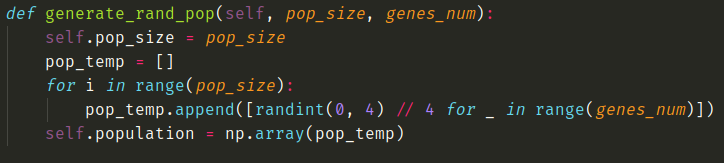
\includegraphics[scale=0.5]{pop_gen_rand_pop}
\end{center}

This method generates a \emph{pop\_size} number of individuals, each having \emph{genes\_num} genes. Genes informs which items are
 present in the knapsack. A gene can be either 0 (item absent) or 1 (item present). There is 80\% chance to get 0 and 20\% to get 1.

\subsubsection{Fitness method}
\begin{center}
	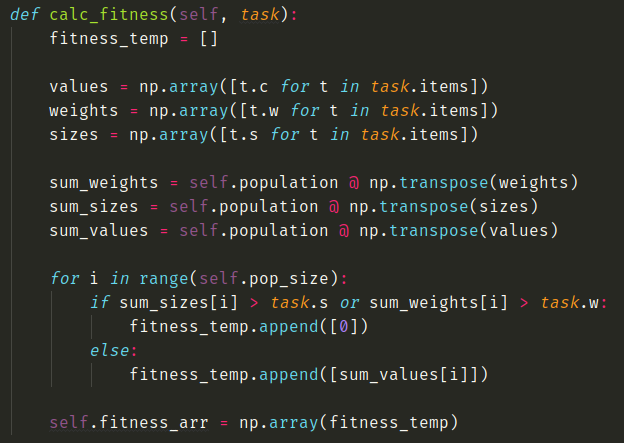
\includegraphics[scale=0.5]{pop_fitness}
\end{center}

At the beginning I split the items stored in the task object into three arrays representing values, weights and sizes. 
Then I do matrix multiplication, as a result of which I get three vectors informing about the total value, weight and size of items in
 the knapsack for each individual. Thanks to NumPy package, such calculations are carried out faster than other methods using loops. 
The fitness values for individuals meeting the task conditions are equal to the sum of the values of the items in their knapsacks.
 Individuals that exceed the maximum values have zeroed values. Results are assigned to the population objects, so that the tournament
  function will not be forced to repeat the calculations during each invocation.


\subsubsection{Get the best individual method}
\begin{center}
	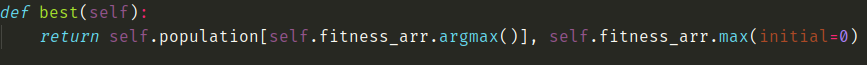
\includegraphics[scale=0.5]{pop_best}
\end{center}

This method returns the best individual and his fitness value.

\subsection{Tournament Function}
\begin{center}
	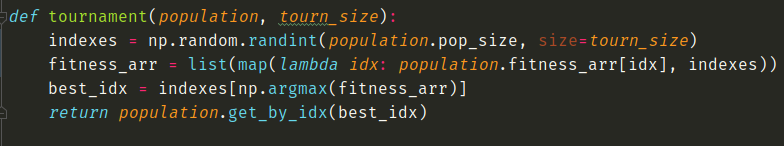
\includegraphics[scale=0.5]{tourn}
\end{center}

This function selects a random slice from the population, retrieves fitness values for that subset and returns the best individual.

\subsection{Crossover Function}
\begin{center}
	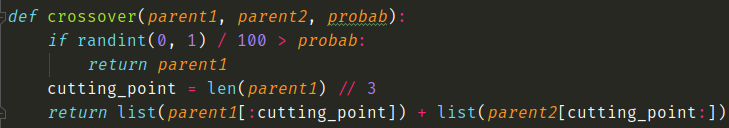
\includegraphics[scale=0.5]{cross}
\end{center}

In the beginning a real number from the range [0, 1] is drawn. If that number is bigger than the given probability, no crossover occurs and the first parent is returned. Otherwise, a child is formed from clippings from both parents.

\subsection{Mutation Function}
\begin{center}
	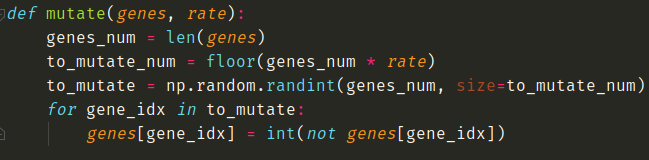
\includegraphics[scale=0.5]{mutate}
\end{center}

The function selects random genes from an individual and converts their values to the opposite, then returns the mutated individual.

\subsection{Mutation Function}
\begin{center}
	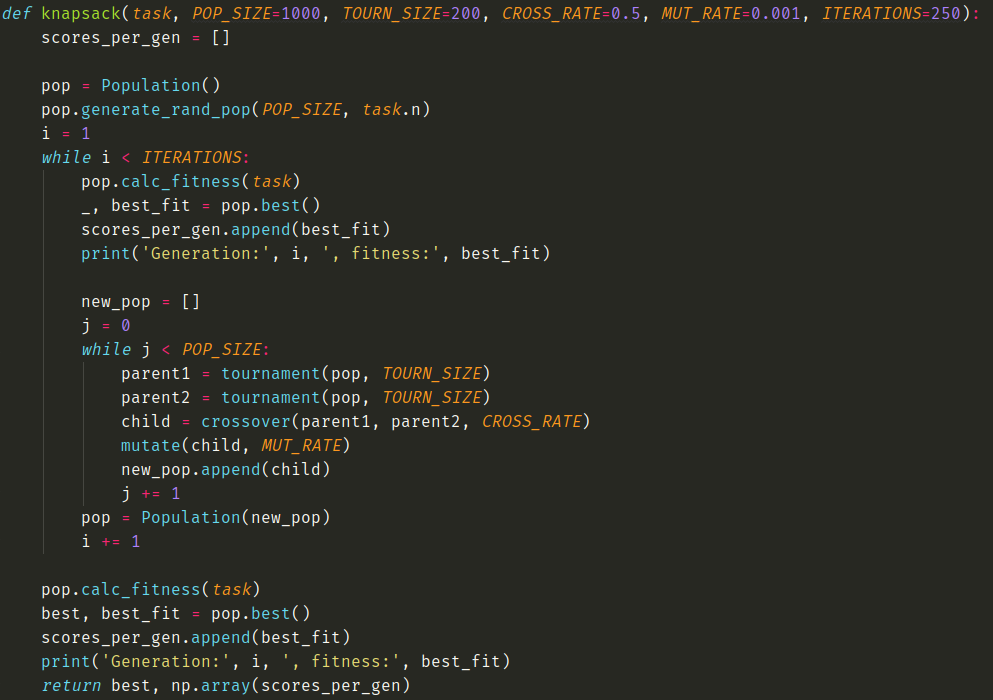
\includegraphics[scale=0.5]{knapsack}
\end{center}

This function combines the others to find the best solution for the given knapsack problem. First, a random population is initiated. 
The creation of new generations will be carried out until the final condition is met. In this case the goal is to reach the given number of iterations. Two parents are selected using the tournament function. They are combined using the crossover function. A newly created child is mutated and stored in a new population. The best fitness value for each iteration is stored in the \emph{scored\_per\_gen} list. The function returns the best individual from the last generation and the array \emph{scored\_per\_gen}.

\section{Analysis of the impact of the parameters}
\end{document}